% Developability, order and holonomy: geometric quality checks for virtually unrolled Herculaneum papyri
% Zinuo Shi, Wellesley College. Working draft; sections live in sections/ so the document can grow.
% Build: latexmk -pdf main.tex   (figures are read from ../docs/figures)
\documentclass[11pt,a4paper]{article}
\usepackage[margin=2.4cm]{geometry}
\usepackage{amsmath,amssymb,amsthm}
\usepackage{graphicx}
\graphicspath{{../docs/figures/}{figures/}}
\usepackage{booktabs}
\usepackage{siunitx}
\sisetup{detect-all,range-phrase=--,range-units=single}
\usepackage[dvipsnames]{xcolor}
\usepackage{caption}
\captionsetup{font=small,labelfont=bf}
\usepackage{enumitem}
\setlist{nosep,leftmargin=*}
\usepackage[colorlinks=true,linkcolor=NavyBlue,citecolor=NavyBlue,urlcolor=NavyBlue]{hyperref}
\usepackage[capitalise,noabbrev]{cleveref}
\usepackage{microtype}

\newtheorem{proposition}{Proposition}
\newtheorem{lemma}{Lemma}
\theoremstyle{remark}
\newtheorem{remark}{Remark}

\newcommand{\todo}[1]{\textcolor{BrickRed}{[TODO: #1]}}
\newcommand{\code}[1]{\texttt{#1}}
\newcommand{\um}{\si{\micro\metre}}
\newcommand{\psifour}{\psi_4}
\DeclareMathOperator{\corr}{corr}
\DeclareMathOperator{\AUC}{AUC}
\DeclareMathOperator{\atantwo}{atan2}

\title{Developability, order and holonomy:\\ geometric quality checks for virtually unrolled Herculaneum papyri}
\author{Zinuo Shi\\ \small Wellesley College \quad \href{https://github.com/ZinuoS/Vesuvius_ZS}{github.com/ZinuoS/Vesuvius\_ZS}}
\date{Working draft, 14 October 2026}

\begin{document}
\maketitle

\begin{abstract}
Virtual unrolling of the Herculaneum papyri produces surface meshes that sometimes drift from one winding of the scroll to the next. Such sheet switches are the dominant failure mode of automated segmentation and are usually caught by eye. This note reports an end-to-end, logged, CPU-only pipeline for PHerc1447 (seed selection, mesh growth, surface rendering, cross-section QA and ink inference on Apple Silicon) together with two geometric quality measures borrowed from physics. The first treats the mesh as a Riemannian surface and asks whether it is developable: the holonomy of parallel transport around small loops, computed as a sum of discrete angle deficits via Gauss--Bonnet, should vanish for a sheet of papyrus. It does, even across a sheet switch, and we show why: the switch is extrinsic, so intrinsic curvature cannot see it. The second treats the papyrus weave as a two-dimensional tetratic phase and measures its order parameter $\psifour=\langle e^{4i\theta}\rangle$ and the quantised disclination charge of its orientation field. Tetratic order separates a sheet switch from clean weave where the standard structure-tensor coherence does not. We also calibrate the released ink-detection models against the team's PHerc.172 w087 map and report a depth-window scan with block-bootstrap confidence intervals. Code, meshes, logs and figures are public.

\end{abstract}

\section{Introduction}
\label{sec:intro}

The Vesuvius Challenge asks for text read from X-ray micro-CT volumes of carbonised scrolls without opening them \cite{seales2023,scrollprize}. The published route has three stages: segment a surface mesh that follows one winding of the rolled sheet, render the CT intensity in a thin slab around that mesh into a flat image stack, and run an ink-detection network on the stack. Stage one is the bottleneck. A tracer grown from a seed point will, with some probability per unit area, cross the interstitial gap and continue on the neighbouring winding. The resulting mesh is smooth, its rendering looks like papyrus, and only the fibre pattern or a cross-section reveals that the surface now covers two different sheets. The organisers' own criterion for unwrapping work is that \emph{visible papyrus fibres do not jump across sheets} \cite{scrollprize}.

This note has two aims. The first is documentary: a complete, headless, timed run of the open-source tools on PHerc1447 from a laptop with no CUDA device, including the failures, so that the next person starts from a working baseline. The second is methodological. Both quality checks introduced here come from physics rather than from image processing, and both are stated with their derivations so that they can be criticised at the level of the equations.

\paragraph{Developability.} A sheet of papyrus is, to the precision of the scan, an isometric embedding of a flat rectangle. Its Gaussian curvature vanishes, so parallel transport of a tangent vector around any closed loop on it returns the vector unchanged. This is the same statement as the Thomas precession of a gyroscope or the Foucault pendulum: the holonomy angle equals the integrated curvature enclosed by the loop. \Cref{sec:holonomy} turns this into a per-loop test on a quad mesh via the discrete Gauss--Bonnet theorem, and reports a negative result with a reason: a sheet switch is a change of \emph{which} surface the mesh follows, not a change of the mesh's intrinsic geometry.

\paragraph{Tetratic order.} The papyrus weave consists of two orthogonal families of fibres, recto and verso. An orientation field with this symmetry is a tetratic, the four-fold analogue of a nematic liquid crystal \cite{degennes}. \Cref{sec:tetratic} defines the order parameter $\psifour$ on tiles of a flattened render and the disclination charge of its phase, and shows that $|\psifour|$ drops from \numrange{0.6}{0.8} on clean weave to \numrange{0.1}{0.3} across a sheet switch, while the structure-tensor coherence that one would normally use stays flat.

\paragraph{Ink detection on a laptop.} \Cref{sec:ink} describes inference with the released \code{ink\_9um} and Hecate checkpoints on the Apple Metal backend, a positive control on PHerc.172 segment w087 against the team's published ink map, a scan of the model's 17-layer depth window through a 28-layer render, and a failed lock-in idea. All of it is scored with Pearson correlation and a Mann--Whitney AUC, with block-bootstrap intervals, so that the differences between settings can be read as evidence rather than as impressions.

The document is a working draft. Sections are written so that results can be appended as the cluster runs described in \cref{sec:discussion} complete.

\section{A headless pipeline on a laptop}
\label{sec:pipeline}

\subsection{Setup}
Everything in this section ran on a MacBook Air (Apple Silicon, 16\,GB) on 14 October 2026, streaming data from \code{s3://vesuvius-challenge-open-data}. The target is PHerc1447, volume \code{20250521151220} at \SI{8.64}{\um}, with the organisers' April 2026 surface prediction (\code{surface-m7-L0-}\allowbreak\code{th0.2}) as the seed field. The command-line tools \code{vc\_grow\_seg\_from\_seed} and \code{vc\_render\_tifxyz} are taken from the VC3D application bundle (build \code{afdb836}, 14 October 2026); ink inference uses the \code{vesuvius} package from the ScrollPrize \code{villa} repository (commit \code{5432721}) in a slim virtual environment with PyTorch on the Metal (MPS) backend and no compiled extensions. Every run is driven by a shell script that logs the command, the build and the wall time.

\subsection{Seeds}
Seeds are drawn from the level-3 pyramid of the surface prediction (\SI{1}{/8} resolution, about \SI{2}{MB} read), uniformly at random with a minimum separation of 600 voxels. Two things went wrong before anything grew.

\begin{enumerate}
\item Seeding from the vertices of the team's May 2025 patches put the tracer off the April 2026 prediction (the prediction value at those vertices was zero). The tracer then started in the gap and produced swirling, sheet-crossing patches. Seeds must come from the \emph{current} prediction.
\item The first prediction-only seed grew \SI{1.35}{cm^2} in \SI{534}{s} and rendered to all zeros: it lay outside the masked scroll. Counting at level 3, the prediction has $39.5\times10^6$ surface voxels, of which only $13.2\times10^6$ (34\,\%) sit where the masked CT exceeds 20. Two thirds of the surface field is outside the object it is meant to describe. A CT mask was added to the seed picker.
\end{enumerate}

\subsection{Grow, render, inspect}
\Cref{tab:seeds} lists the seeds grown with the tracer at 35 generations and rendered as 28 layers at step 1 (the window the \SI{9}{\um} ink model expects). \code{composite.py} writes a maximum-intensity projection, the middle layer and a contact sheet; \code{qa.py} samples a $3\times3$ grid of mesh points and draws the CT cross-sections through each with the mesh overlaid (\cref{fig:contact}). The cross-sections caught a failure the flattened images did not: for seed 5452 the top third of a visually clean patch lies in air, where the tracer overgrew the outer wrap.

\begin{table}[t]
\centering\small
\caption{Patches grown on PHerc1447. Grow time is for \code{vc\_grow\_seg\_from\_seed} alone. Verdicts are from the contact sheet and the cross-section QA.}
\label{tab:seeds}
\begin{tabular}{@{}lrl@{}}
\toprule
seed $(x,y,z)$ & grow [s] & verdict \\
\midrule
5452 4100 22772 & 107 & clean weave; top third in air \\
3532 4492 23020 & 375 & clean; sheet switch, lower left \\
2388 3356 22308 & 212 & mixed \\
3092 6212 22708 & 76  & mixed \\
7036 4612 24060 & 167 & reject: compressed mass \\
4020 1948 24284 & 63  & reject: edge, 11\,\% fill \\
4144 2742 12557 & 145 & announced text site; 9/9 QA points on sheet \\
\bottomrule
\end{tabular}
\end{table}

\begin{figure}[t]
\centering
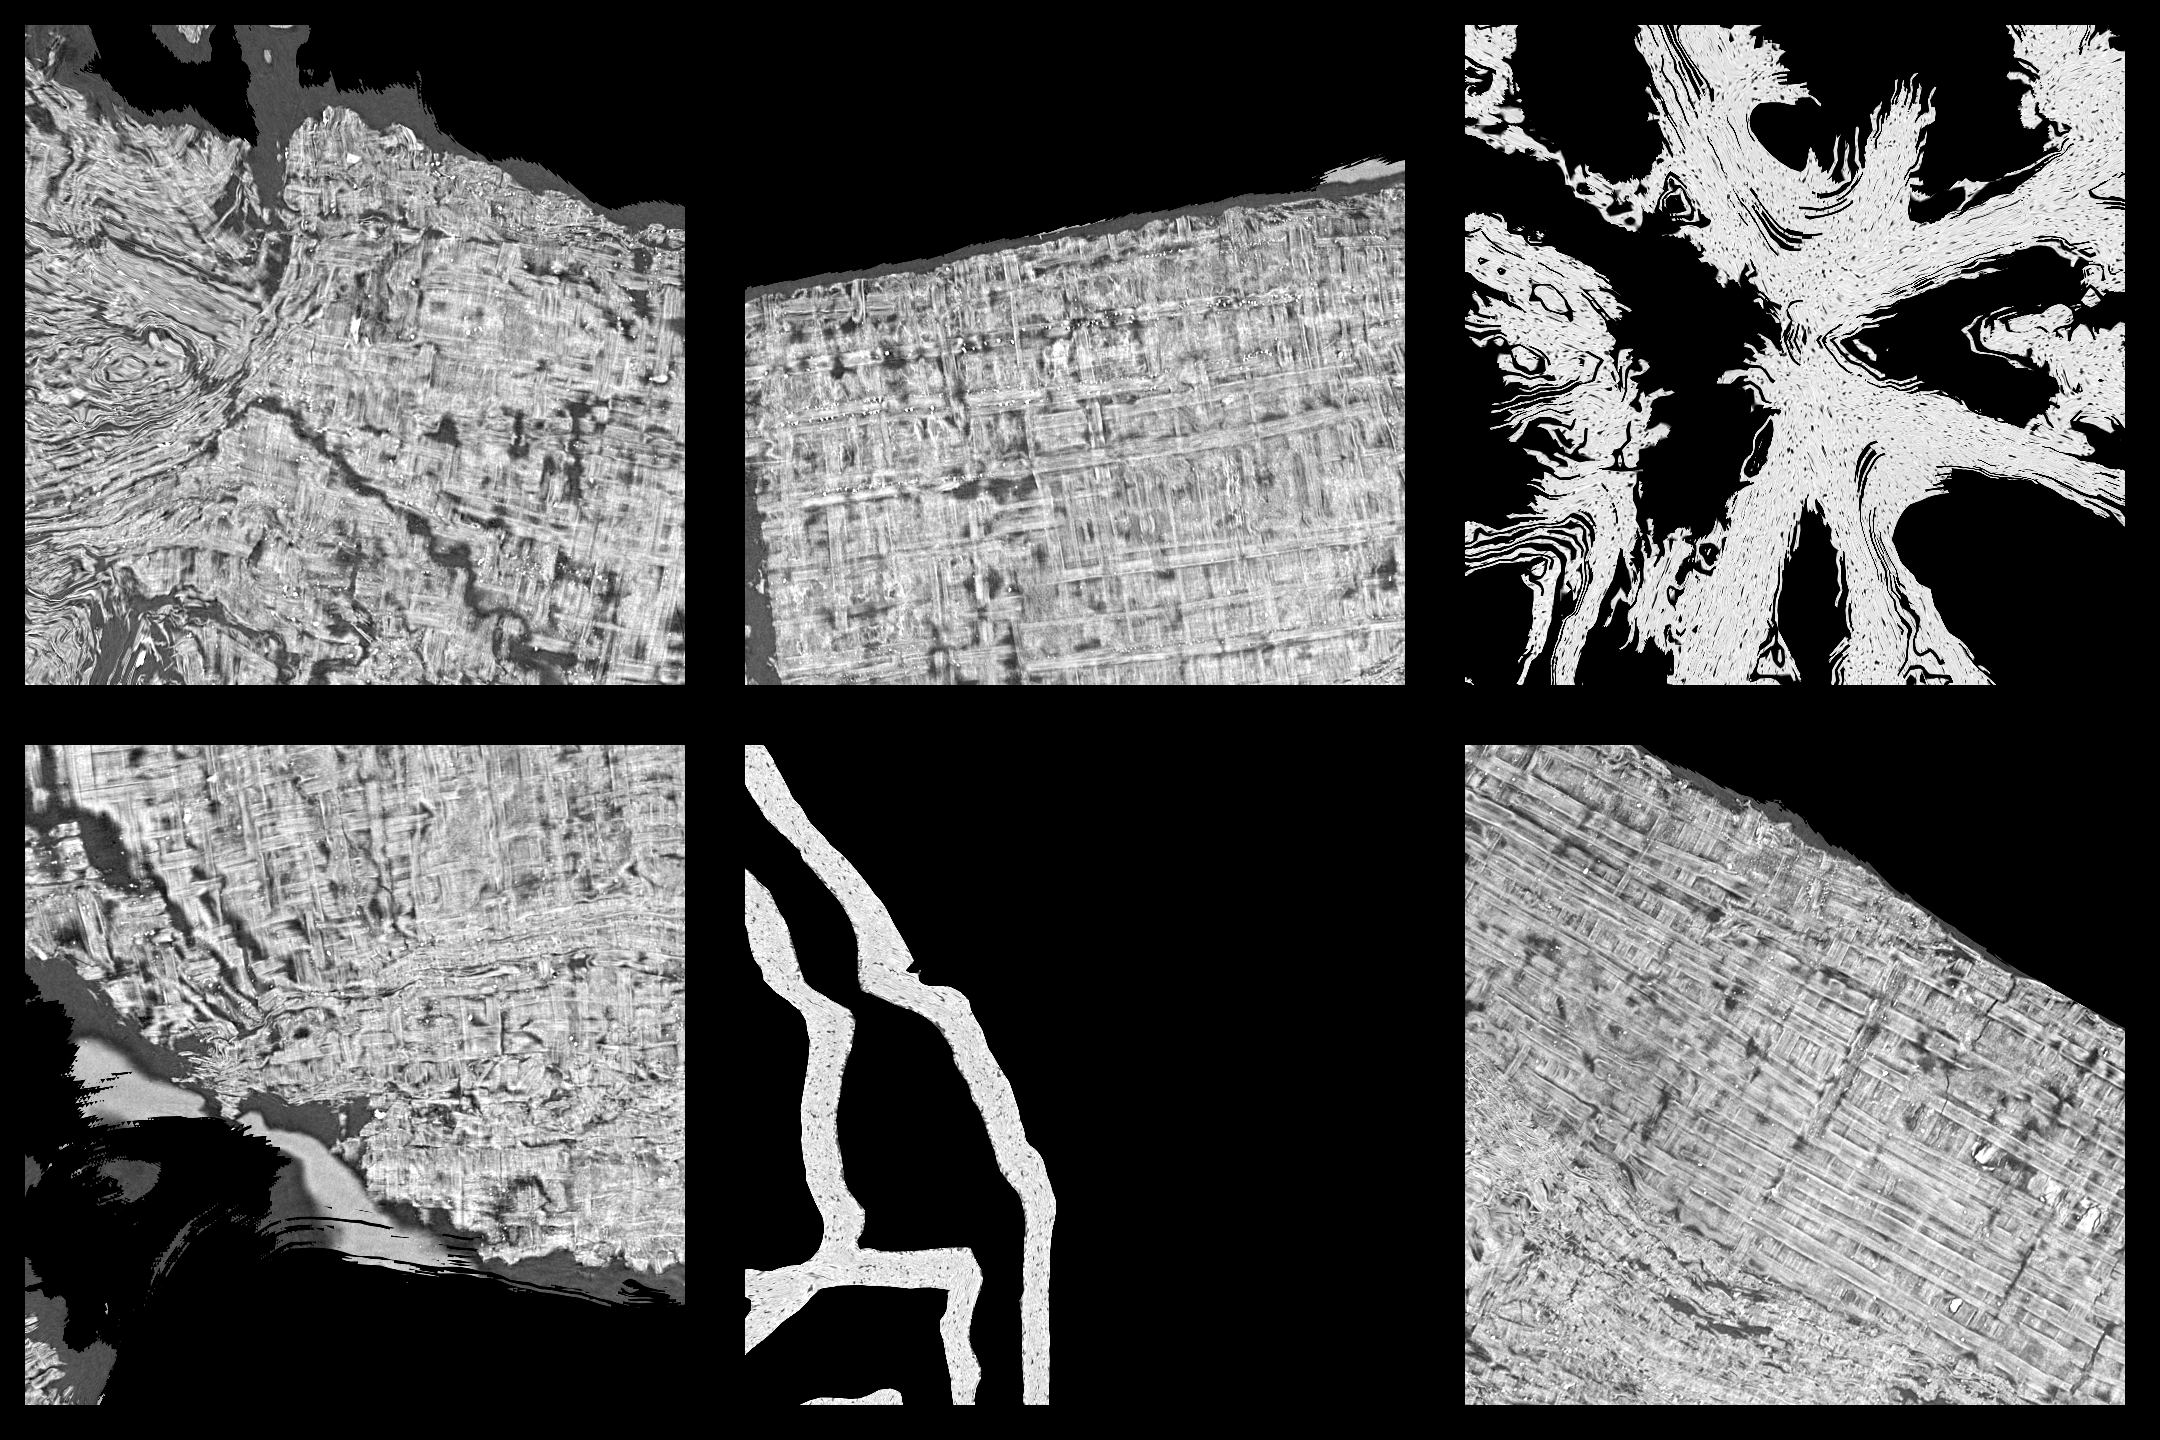
\includegraphics[width=\linewidth]{_contact_run3}
\caption{Contact sheet for the six in-scroll seeds of the third run (middle layer of each render). Two are clean, two mixed, two rejected. The lower-left region of 3532 is the sheet switch analysed in \cref{sec:holonomy,sec:tetratic}.}
\label{fig:contact}
\end{figure}

\paragraph{Failure modes found.} Stale seeds off the current prediction; prediction voxels outside the scroll mask; overgrowth into air past the outer wrap; and the sheet switch that motivates the rest of this note.

\section{Developability and holonomy}
\label{sec:holonomy}

\subsection{Physical motivation}
A vector parallel-transported around a closed loop on a curved surface comes back rotated. The rotation angle is the holonomy of the loop, and on a two-dimensional surface it is fixed by the Gaussian curvature enclosed:
\begin{equation}
\Phi(\partial D) = \iint_D K\,\mathrm{d}A \pmod{2\pi}.
\label{eq:holonomy}
\end{equation}
This single identity underlies the Foucault pendulum (the swing plane precesses by $2\pi\sin\varphi$ per day, the solid angle of the polar cap above latitude $\varphi$ on the unit sphere, $K=1$), the geometric phase of a spin, and Thomas precession, where the loop is drawn on the hyperboloid of velocities ($K=-1$) and the precession per orbit is the enclosed hyperbolic area \cite{rhodes2004}. The physics is always the same: the loop samples the curvature it encloses.

A sheet of papyrus is a developable surface. It was manufactured flat and, however it was rolled, crushed and carbonised, the rolling is to good approximation an isometry: the sheet bends but does not stretch. Developable means $K=0$ everywhere, so by \cref{eq:holonomy} every loop on it has zero holonomy. The hope was that a mesh which leaves one winding for the next would have to curve to do so, acquire $K\neq0$ in the transition, and announce the switch through a non-zero holonomy that a purely metric check could not see. The hope was wrong, for a reason given in \cref{sec:holonomy-why}, but the test is cheap, exact and worth stating.

\subsection{Discrete formulation on a quad mesh}
The tracer writes a quad mesh as three images $X,Y,Z$ of shape $H\times W$: vertex $(i,j)$ sits at $\mathbf{v}_{ij}=(X_{ij},Y_{ij},Z_{ij})$ in voxel coordinates, with nominal grid step $s$ voxels (from \code{meta.json}, $s=1/\text{scale}$). At an interior vertex $\mathbf{v}$ with four neighbours $\mathbf{n}_1,\dots,\mathbf{n}_4$ in cyclic order (up, right, down, left), define the umbrella angles and the angle deficit
\begin{equation}
\theta_k=\arccos\frac{(\mathbf{n}_k-\mathbf{v})\cdot(\mathbf{n}_{k+1}-\mathbf{v})}{|\mathbf{n}_k-\mathbf{v}|\,|\mathbf{n}_{k+1}-\mathbf{v}|},
\qquad
\delta(\mathbf{v})=2\pi-\sum_{k=1}^{4}\theta_k .
\label{eq:deficit}
\end{equation}
On a flat sheet the four angles sum to $2\pi$ and $\delta=0$. On a smooth surface sampled at step $s$ the deficit equals the curvature integrated over the vertex's dual cell,
\begin{equation}
\delta(\mathbf{v})=\iint_{A_{\mathbf{v}}}K\,\mathrm{d}A+O(s^{3}),
\label{eq:deficit-K}
\end{equation}
which is the discrete Gauss--Bonnet theorem for piecewise-flat surfaces \cite{meyer2003}; the derivation for the umbrella is in \cref{app:gaussbonnet}. Summing \cref{eq:deficit-K} over the vertices enclosed by a loop recovers \cref{eq:holonomy}. We take loops to be the boundaries of $L\times L$ blocks of cells and define the loop holonomy
\begin{equation}
\Phi_L(a,b)=\sum_{\mathbf{v}\in \text{block}(a,b)}\delta(\mathbf{v}),
\label{eq:loop}
\end{equation}
with $L=6$, so each loop encloses $6s$ voxels $\approx\SI{1}{mm}$ on a side at \SI{8.64}{\um} and the \code{scale} of these meshes. A vertex with any invalid neighbour (zero coordinates) is excluded, and a block containing an excluded vertex is dropped.

\paragraph{Baseline.} The existing metric check is parametrisation stretch. With edge lengths $e^{x}_{ij}=|\mathbf{v}_{i,j+1}-\mathbf{v}_{ij}|/s$ and $e^{y}_{ij}=|\mathbf{v}_{i+1,j}-\mathbf{v}_{ij}|/s$, an isometric parametrisation has $e\equiv1$, and we report per block
\begin{equation}
\sigma_L(a,b)=\max_{\text{block}}\bigl|\log e\bigr| .
\label{eq:stretch}
\end{equation}
Stretch is sensitive to the tracer's parametrisation; holonomy, by \cref{eq:holonomy}, is invariant under reparametrisation and sees only the embedded surface. The two should therefore disagree exactly where the geometry, rather than the parametrisation, is wrong.

\subsection{Result}
\code{holonomy.py} computes \cref{eq:deficit,eq:loop,eq:stretch} for a patch in under a second and writes a three-panel figure (flattened mid layer, $|\Phi_6|$, $\sigma_6$). Across the patches of \cref{tab:seeds}:
\begin{itemize}
\item $|\Phi_6|$ ranks the patches in the order the eye does: the announced text site 4144 is cleanest, 3532 worst. \todo{insert median / p90 / p99 of $|\Phi_6|$ in degrees per patch from \code{holonomy.py}}
\item Over blocks, $\corr(|\Phi_6|,\sigma_6)$ lies between 0.60 and 0.84 per patch. Most of what holonomy flags, stretch already flags.
\item $|\Phi_6|$ is \emph{blind} to the sheet switch in the lower left of 3532 (\cref{fig:contact}). The blocks over the switch are no more curved than the clean weave beside them.
\end{itemize}
Holonomy is retired as a sheet-switch detector and kept as a finding. The reason is instructive.

\subsection{Why intrinsic curvature cannot see a sheet switch}
\label{sec:holonomy-why}
Let $S_0$ be a developable surface, the winding the tracer started on, with unit normal $\mathbf{n}$. The next winding $S_t$ is, locally, an offset surface $S_0+t\,\mathbf{n}$ at the interstitial gap $t$ (of order \SIrange{50}{150}{\um} in these scrolls). The curvature of an offset surface follows from the shape operator: if $\kappa_1,\kappa_2$ are the principal curvatures of $S_0$, those of $S_t$ are $\kappa_i/(1-t\kappa_i)$, hence
\begin{equation}
K_t=\frac{K}{1-2Ht+Kt^{2}}, \qquad H=\tfrac12(\kappa_1+\kappa_2).
\label{eq:offset}
\end{equation}
With $K=0$ the numerator vanishes and $K_t=0$: every offset of a developable surface is developable. The windings form a one-parameter family of flat surfaces, and nothing intrinsic distinguishes them.

Now let the tracer drift between them. Its output is a smooth embedding $\mathbf{f}=S_0+h\,\mathbf{n}$ with a displacement field $h(u,v)$ that rises from $0$ to $t$ across a transition region. Work in the tangent frame of $S_0$ where, since $S_0$ is flat, the problem reduces locally to the graph of $h$ over the plane, with
\begin{equation}
K_h=\frac{h_{uu}h_{vv}-h_{uv}^{2}}{\bigl(1+h_u^{2}+h_v^{2}\bigr)^{2}} .
\label{eq:graph}
\end{equation}
A tracer that crosses the gap along a front, $h=h(u)$ only, has $h_{vv}=h_{uv}=0$ and $K_h\equiv0$: the ramp between the sheets is a generalised cylinder, developable, with zero holonomy around every loop. Only a ramp that bends in both directions carries curvature, and its size is set by the gap and the transition length $\ell$: $h_{uu}\sim h_{vv}\sim t/\ell^{2}$, so $K_h\sim t^{2}/\ell^{4}$ and the holonomy of an $\ell\times\ell$ loop is
\begin{equation}
\Phi\sim K_h\,\ell^{2}\sim\Bigl(\frac{t}{\ell}\Bigr)^{2}\approx\Bigl(\frac{0.1\,\text{mm}}{1\,\text{mm}}\Bigr)^{2}=10^{-2}\ \text{rad}\approx0.6^{\circ},
\label{eq:estimate}
\end{equation}
below the deficit noise of a mesh whose vertices are placed to a voxel. The switch is a change in \emph{which} sheet the surface follows, a property of the CT scalar field along $\mathbf{n}$. It is extrinsic. Holonomy, by \cref{eq:holonomy}, measures the intrinsic metric and is the wrong instrument by construction. The right instrument has to look at what is painted on the surface, which is the subject of \cref{sec:tetratic}, or at the intensity profile along the normal, which is the per-tile re-localisation proposed in \cref{sec:discussion}.

\begin{remark}
The same argument explains why stretch and holonomy correlate at all: where the tracer's parametrisation is distorted, the vertices are also noisy, and noisy vertices produce spurious deficits. Holonomy on these meshes is a noise meter for vertex placement, not a curvature meter. A smoothed mesh would decorrelate the two but would not create the missing signal.
\end{remark}

\section{Tetratic order of the weave and its disclinations}
\label{sec:tetratic}

\subsection{Physical motivation}
If intrinsic geometry cannot see a sheet switch, the texture painted on the surface can. Papyrus is a laminate of two layers of parallel strips laid at right angles, so a flattened render of a single sheet shows two orthogonal fibre families with a well-defined local axis. An orientation field that is invariant under rotation by $\pi/2$ is, in the language of soft matter, a tetratic: the four-fold cousin of the nematic phase of a liquid crystal, whose director is invariant under $\pi$ \cite{degennes}. The natural order parameter is therefore not the nematic $\langle e^{2i\theta}\rangle$ but
\begin{equation}
\psifour=\bigl\langle e^{4i\theta}\bigr\rangle ,
\label{eq:psi4}
\end{equation}
and the natural defects are disclinations of the director field with charge quantised in units of $1/4$. The claim to be tested: a legible sheet has $|\psifour|$ near one; where the mesh crosses between windings, or renders a blend of two sheets, the orientation field loses long-range order and $|\psifour|$ collapses, even though the local texture may remain anisotropic.

\subsection{Orientation field from the structure tensor}
Let $I(\mathbf{x})$ be the middle layer of a render. Smooth and differentiate, $\mathbf{g}=\nabla(G_{\sigma}*I)$ with $\sigma=2$ px, and form the structure tensor by averaging the outer product over a window $w=6$ px,
\begin{equation}
\mathbf{J}=G_{w}*\bigl(\mathbf{g}\mathbf{g}^{\mathsf T}\bigr)=
\begin{pmatrix}J_{xx}&J_{xy}\\ J_{xy}&J_{yy}\end{pmatrix}.
\label{eq:J}
\end{equation}
Its eigenvalues and the orientation of the dominant gradient are
\begin{equation}
\lambda_{\pm}=\tfrac12\bigl(J_{xx}+J_{yy}\bigr)\pm\tfrac12\sqrt{(J_{xx}-J_{yy})^{2}+4J_{xy}^{2}},
\qquad
\theta=\tfrac12\atantwo\bigl(2J_{xy},\,J_{xx}-J_{yy}\bigr),
\label{eq:theta}
\end{equation}
with $\theta$ defined modulo $\pi$. The standard measure of local anisotropy is the coherence
\begin{equation}
c=\frac{\lambda_{+}-\lambda_{-}}{\lambda_{+}+\lambda_{-}}
=\frac{\sqrt{(J_{xx}-J_{yy})^{2}+4J_{xy}^{2}}}{J_{xx}+J_{yy}}\in[0,1].
\label{eq:coherence}
\end{equation}
Two remarks fix the symmetry. First, $\theta$ in \cref{eq:theta} is the gradient direction, perpendicular to the fibre; but $e^{4i(\theta+\pi/2)}=e^{4i\theta}$, so the tetratic order parameter does not care, and neither does it care which of the two fibre families dominates a pixel. Second, a nematic parameter would fail here for a structural reason: a balanced weave with fractions $p$ and $1-p$ of pixels on the two families has $|\langle e^{2i\theta}\rangle|=|2p-1|$, which vanishes at $p=\tfrac12$ for a perfectly ordered sheet, whereas $|\psifour|=1$ for any $p$.

\subsection{Order parameter and charge per tile}
Divide the render into $T\times T$ tiles ($T=128$ px, about \SI{1.1}{mm}) and keep tiles that are at least 95\,\% inside the valid render. Per tile,
\begin{equation}
\psifour=\frac{1}{T^{2}}\sum_{\mathbf{x}\in\text{tile}}e^{4i\theta(\mathbf{x})},\qquad
\bar c=\frac{1}{T^{2}}\sum_{\mathbf{x}\in\text{tile}}c(\mathbf{x}).
\end{equation}
$|\psifour|$ measures whether the orientations across a millimetre agree; $\bar c$ measures whether each pixel is locally striped. They are different quantities. A polydomain texture, or a render in which two sheets with different weave axes overlap, is locally anisotropic and globally disordered: high $\bar c$, low $|\psifour|$. For two overlapping sheets with axes differing by $\Delta$ and equal weight, $|\psifour|=\bigl|\tfrac12(1+e^{4i\Delta})\bigr|=|\cos2\Delta|$, which vanishes at $\Delta=45^{\circ}$.

The disclination charge enclosed by a tile is the winding of the tetratic phase around its boundary. Write $z_4(\mathbf{x})=e^{4i\theta(\mathbf{x})}$ and let $\phi=\arg\bigl(G_{16}*z_4\bigr)$ be the phase of the complex field smoothed over 16 px (smoothing the complex field, not the angle, avoids branch cuts). Then
\begin{equation}
q=\frac{1}{2\pi}\oint_{\partial\text{tile}}\mathrm{d}\phi\in\mathbb Z ,
\label{eq:charge}
\end{equation}
evaluated as the sum of wrapped finite differences of $\phi$ around the tile boundary. Since $\phi=4\theta$ where the field is ordered, an integer winding $q$ of $\phi$ is a winding $q/4$ of the director: the charge is quantised in quarters, as a tetratic requires. The phase is undefined where $|G_{16}*z_4|\to0$, so $q$ is counted only on tiles with $|\psifour|\ge0.25$.

\subsection{Results}
\code{tetratic.py} runs in a few seconds per render. The findings, in order of confidence:
\begin{enumerate}
\item \textbf{Order separates the switch.} In patch 3532, tiles over the lower-left sheet switch have $|\psifour|$ between 0.1 and 0.3; tiles over clean weave have 0.6 to 0.8. Over the same tiles the coherence $\bar c$ is flat at \numrange{0.4}{0.6}. Local anisotropy is not order, and the standard check would not have flagged the region.
\item \textbf{Raw winding is noise; regularised winding is usable.} Counting the winding of the unsmoothed $4\theta$ marks 70--85\,\% of tiles as charged. With the smoothed phase and the $|\psifour|$ floor the fraction of charged tiles is 3.9\,\% (5452), 12.7\,\% (3532), 32\,\% (4144) and 19--23\,\% (the two w087 control crops). The ordering is the ordering of visible damage and sheet mixing.
\item \textbf{Medians across tiles.} $|\psifour|$: 3532 0.52, 5452 0.46, the team's 1447 patch 0.39, the 4144 text site 0.32, w087 crops 0.30 and 0.30. The overall median of 3532 is high because most of it is clean; the switch is a local minimum, which is the point of a per-tile map.
\item \textbf{Not an ink signature.} $\corr(|\psifour|,\text{team ink map})=+0.05$ on both w087 crops, with bootstrap intervals that include zero. Order measures the weave, not the writing.
\end{enumerate}

\paragraph{Caveats.} $|\psifour|$ is a weave-legibility score. It falls where the sheet is damaged (the 4144 site), not only where the mesh switches sheet, and its absolute level differs between scans (the w087 control was scanned at \SI{7.91}{\um}, 1447 at \SI{8.64}{\um}), so it should be used as a within-render map and contrast, not as a universal threshold. A switch that preserves the weave axis to within a few degrees would also preserve $|\psifour|$; the disclination map and the normal-profile test of \cref{sec:discussion} are the complements.

\todo{figure: four-panel \code{\_tetratic.png} for 3532 (mid layer, $|\psifour|$, $q$, $\bar c$); copy from \code{renders/} to \code{docs/figures/}}

\section{Ink detection: calibration, depth window and a failed lock-in}
\label{sec:ink}

\subsection{Inference on Apple Silicon}
The released \code{ink\_9um} checkpoint (\code{hybrid\_3d2d-seed42/step-075000}) runs on the Metal backend from a virtual environment containing only the packages that \code{vesuvius.ink\_detection.inference} imports (PyTorch 2.14, no nnU-Net, no MONAI, no compiled extensions). A 28-layer render of a \SI{1.4}{mm}-scale patch takes \SIrange{86}{138}{s} per direction. On the PHerc1447 patches 5452 and 3532, and on the three patches at the announced text site around $(4144,2742,12557)$, the model returns blobs with no strokes and no rows in either direction. The organisers reported about ten letters at that site on 24 September 2026 with a new \SI{9}{\um} recipe and a fine-tuned model, so the released weights, not the pipeline, are the limiting factor on this scroll.

\subsection{Positive control and scoring}
To separate pipeline errors from model weakness, the same renderer flags and the same inference script were run on PHerc.172 segment w087, for which the team has published an ink map at $1/8$ scale. Two $2048\times2048$ crops at render origin $(5440,5120)$ and $(1200,9200)$ were rendered from the published mesh (\SI{7.91}{\um} volume).

A prediction $p$ at full resolution is compared with the team map $t$ on the team's grid by block-averaging, $q_{ab}=\frac1{64}\sum_{8a\le i<8a+8}\sum_{8b\le j<8b+8}p_{ij}$. Two scores are reported:
\begin{align}
\corr &=\frac{\sum(q-\bar q)(t-\bar t)}{\sqrt{\sum(q-\bar q)^{2}\sum(t-\bar t)^{2}}},\label{eq:corr}\\
\AUC &=\frac{1}{n_{+}n_{-}}\sum_{i\in+}\sum_{j\in-}\mathbf 1[q_i>q_j]
=\frac{R_{+}-n_{+}(n_{+}+1)/2}{n_{+}n_{-}},\label{eq:auc}
\end{align}
where the positive set is the top 15\,\% of the team map, $R_{+}$ is the rank sum of the predictions on that set, and the second form is the Mann--Whitney identity used in \code{bench172.py}. The AUC is the probability that a randomly chosen ink pixel is scored above a randomly chosen non-ink pixel; 0.5 is chance.

\Cref{tab:control} gives the control numbers. The pipeline is sound: the reverse direction (the inked face) correlates at \numrange{0.36}{0.40} with the team map on the first crop; the forward direction is near zero, as it should be.

\begin{table}[t]
\centering\small
\caption{Positive control on PHerc.172 w087 against the team's published ink map. Pearson correlation and AUC per \cref{eq:corr,eq:auc}; rev is the inked side. Hecate ran at stride 64; the fair stride-32 comparison is pending (\cref{sec:discussion}).}
\label{tab:control}
\begin{tabular}{@{}llcccc@{}}
\toprule
& & \multicolumn{2}{c}{crop $(5440,5120)$} & \multicolumn{2}{c}{crop $(1200,9200)$}\\
\cmidrule(lr){3-4}\cmidrule(lr){5-6}
model & window & corr rev / fwd & AUC rev / fwd & corr rev / fwd & AUC rev\\
\midrule
ink\_9um & S6 (default) & 0.363 / 0.053 & 0.727 / 0.566 & 0.240 / 0.021 & --\\
ink\_9um & S2 & 0.398 / 0.102 & 0.746 / -- & 0.266 / $-0.007$ & 0.688\\
Hecate \SI{9.6}{\um} & stride 64 & 0.240 / 0.102 & 0.706 / 0.602 & not run & \\
\bottomrule
\end{tabular}
\end{table}

\subsection{Depth-window scan with block bootstrap}
The model consumes 17 of the 28 rendered layers. Let $S$ be the index of the first layer; the default is $S=6$, the centred window. Sliding $S$ through $\{0,2,4,6,8,10,11\}$ on the first crop (reverse direction) gives correlations
\[
0.341,\ 0.398,\ 0.391,\ 0.363,\ 0.370,\ 0.286,\ 0.248 .
\]
Differences of a few hundredths need an uncertainty. Pixels of an ink map are not independent, so an ordinary bootstrap would understate the variance. We use a block bootstrap: partition the $256\times256$ downsampled maps into $16\times16$ cells, resample cells with replacement 2000 times, recompute $\corr(q_S,t)-\corr(q_6,t)$ on each resample, and take the central 95\,\% interval. The results:
\begin{center}\small
\begin{tabular}{@{}lcccccc@{}}
\toprule
$S$ & 0 & 2 & 4 & 8 & 10 & 11\\
\midrule
$\Delta\corr$ vs $S=6$ & $-0.021$ & $+0.036$ & $+0.028$ & $+0.007$ & $-0.077$ & $-0.115$\\
95\,\% CI & & $[-0.001,+0.073]$ & & & $[-0.125,-0.032]$ & $[-0.171,-0.059]$\\
\bottomrule
\end{tabular}
\end{center}
On the second crop, $S=2,4,6$ give $0.266,0.251,0.240$ and $\Delta_{2-6}=+0.026\ [-0.023,+0.073]$; pooling the two crops, $\Delta_{2-6}=+0.031\ [+0.000,+0.062]$.

\paragraph{Reading.} Three statements of different strength. (i) Moving the window away from the inked face ($S\ge10$) destroys the signal, and the interval excludes zero with room to spare: the ink is near the surface, as expected. (ii) Shifting the window two layers towards the inked face ($S=2$) gains about $0.03$ in correlation, replicated in direction on both crops, with a pooled interval that just excludes zero. It was adopted as the default for this scroll. (iii) The wrong side is dead at all depths, so the forward direction cannot be rescued by re-centring.

\subsection{A lock-in detector that did not work}
Because the forward and reverse predictions are computed from the same slab, structure that appears in both is texture rather than ink: a lock-in amplifier rejects what is common to signal and reference. Define z-scored maps $\tilde r,\tilde f,\tilde t$ and fit $k$ on one crop by least squares on the residual, $\tilde t-\tilde r\approx -k\tilde f$, then test $L=\tilde r-k\tilde f$ on the other crop. Fitted $k$ ranged over \numrange{0.04}{0.17}; $\corr(L,t)$ changed by less than $0.01$ relative to $\corr(\tilde r,t)$ in all four fit/test combinations. A harder two-sided veto, setting $L$ to its minimum wherever both $\tilde f>1$ and $\tilde r>1$, \emph{hurt}: $0.398\to0.312$. The forward map carries a weak copy of the ink (its AUC of 0.566 is above chance), so vetoing on it removes signal. One-sidedness of the ink is a global property of the two maps, not a pixel-wise one, and a pixel-wise reference subtraction has nothing to subtract. Dead, and recorded so that it is not tried again.

\section{Discussion and next steps}
\label{sec:discussion}

\paragraph{What the two geometric checks establish.} The holonomy result is a theorem-shaped negative: by \cref{eq:offset,eq:graph}, a smooth passage between developable windings is itself developable, so no intrinsic quantity, holonomy or otherwise, can detect a sheet switch. Any detector must be extrinsic. The tetratic order parameter is one such detector and it works on the one switch we have, where the standard coherence measure does not. Its limits are stated in \cref{sec:tetratic}: it responds to damage as well as to mixing, and it would miss a switch that preserves the weave axis.

\paragraph{The extrinsic test that follows.} The sheet identity lives in the CT intensity profile along the mesh normal. A 28-layer render already samples that profile at each pixel. The proposal is to fit, per tile, a depth profile $I(z)$ to a template for a single sheet (bright papyrus between dark gaps), and to re-localise the surface to the profile's maximum. Tiles whose best-fit offset drifts continuously from one sheet spacing to the next are on a ramp; tiles whose profile has two maxima are rendering two sheets. This is the per-tile surface re-localisation listed in the notebook and it uses no ground truth. \todo{implement; report on 3532 and 5452}

\paragraph{Surface prediction outside the scroll.} The finding that two thirds of the m7 surface field at level 3 sits where the masked CT is at most 20 is cheap to check at level 2 and with thresholds 10 and 40, and should be, since it changes how seeds are drawn and how much of the prediction is real. \todo{run the robustness check}

\paragraph{Ink detection.} Three cluster runs are queued on the MIT ORCD Engaging cluster (\code{orcd/}): Hecate at stride 32 on both control crops, which is the fair comparison against \code{ink\_9um} (bar: 0.398 / 0.746); the depth-window scan on the second crop at full resolution; and fine-tuning. The fine-tuning plan is to distil onto PHerc.172 with the team's dense map as teacher, hold out whole windings so that train and test never share a sheet, score with \cref{eq:corr,eq:auc}, and only then pseudo-label on 1447 starting from the announced text site. Training and prediction regions must not overlap for a First Letters claim, and the same discipline applies here.

\paragraph{Why a physicist's framing earns its place.} Both measures are order parameters in the Landau sense: a scalar built from a local field, invariant under the symmetry of the phase, that vanishes when the phase is lost. Holonomy is the order parameter of flatness; $\psifour$ is the order parameter of the weave. The negative result for the first and the positive for the second are the same lesson from two sides: the segmentation failure we care about is a failure of \emph{identity}, not of \emph{shape}, and the measure has to be one that identity breaks.

\paragraph{For the conference version.} \todo{related work on segmentation QA in the Vesuvius community (fibre-following, Thaumato, the team's own stitching checks); relation to nematic texture analysis in materials imaging; a second scroll; the normal-profile test with numbers}

\section{Reproducibility}
\label{sec:repro}

All code, grown meshes (\code{patches/}, tifxyz), timed logs (\code{logs/}) and figures are at \url{https://github.com/ZinuoS/Vesuvius_ZS} under the MIT licence. Renders, predictions and checkpoints are regenerated by the scripts; nothing in the repository is required beyond the public bucket and the released weights.

\begin{center}\footnotesize
\begin{tabular}{@{}lp{7.2cm}p{4.2cm}@{}}
\toprule
step & command & wall time on the Air\\
\midrule
environment & \code{./setup\_ink.sh} & minutes (downloads \SI{132}{MB} checkpoint)\\
seeds & \code{python3 seeds.py --z 22000 24600 --n 8} & seconds (reads level 3)\\
grow + render + QA & \code{SEEDS=seeds.txt ./run.sh} & \SIrange{63}{375}{s} grow, minutes render\\
ink inference & \code{./ink.sh seed\_5452\_4100\_22772} & \SIrange{86}{138}{s} per direction\\
positive control & \code{./control.sh 5440 5120} & render + two inferences\\
depth scan & \code{./depthscan.sh ctrl172\_w087\_5440\_5120} & seven inferences\\
holonomy & \code{python3 holonomy.py patches/seed\_3532\_4492\_23020} \code{--L 6} & $<\SI{1}{s}$\\
tetratic & \code{python3 tetratic.py renders/seed\_3532\_4492\_23020\allowbreak\_mid.png} & seconds\\
\bottomrule
\end{tabular}
\end{center}

Two practical notes for anyone repeating this on macOS. A command-line tool taken from the VC3D bundle can be killed at first launch from Terminal with exit 137 (the first-execution check on an ad-hoc-signed binary); \code{run.sh} retries once. And the ink package imports cleanly on MPS without nnU-Net or MONAI if only its runtime dependencies are installed; \code{setup\_ink.sh} lists them, and \code{PYTORCH\_ENABLE\_MPS\_FALLBACK=1} covers the few operators Metal lacks.


\bibliographystyle{plain}
\begin{thebibliography}{9}
\bibitem{seales2023} W.~B. Seales, C.~S. Parker, M. Segal, E. Tov, P. Shor and Y. Porath, From damage to discovery via virtual unwrapping: reading the scroll from En-Gedi, \emph{Science Advances} \textbf{2} (2016) e1601247.
\bibitem{scrollprize} Vesuvius Challenge, Prizes and submission requirements, \url{https://scrollprize.org/prizes}, accessed 14 October 2026.
\bibitem{rhodes2004} J.~A. Rhodes and M.~D. Semon, Relativistic velocity space, Wigner rotation, and Thomas precession, \emph{American Journal of Physics} \textbf{72} (2004) 943--960.
\bibitem{meyer2003} M. Meyer, M. Desbrun, P. Schr\"oder and A.~H. Barr, Discrete differential-geometry operators for triangulated 2-manifolds, in \emph{Visualization and Mathematics III}, Springer (2003) 35--57.
\bibitem{docarmo} M.~P. do Carmo, \emph{Differential Geometry of Curves and Surfaces}, Prentice-Hall (1976).
\bibitem{degennes} P.~G. de Gennes and J. Prost, \emph{The Physics of Liquid Crystals}, 2nd ed., Oxford University Press (1993).
\bibitem{bigun1987} J. Big\"un and G.~H. Granlund, Optimal orientation detection of linear symmetry, in \emph{Proc. IEEE First International Conference on Computer Vision} (1987) 433--438.
\bibitem{villa} ScrollPrize, \code{villa} repository (vesuvius package, ink\_9um and Hecate checkpoints), \url{https://github.com/ScrollPrize/villa}, commit \code{5432721}.

\end{thebibliography}

\appendix
\section{Derivations}
\label{app:derivations}

\subsection{Holonomy equals enclosed curvature}
\label{app:holonomy}
Let $D\subset S$ be simply connected with piecewise-smooth boundary $\gamma=\partial D$, and let $(\mathbf e_1,\mathbf e_2)$ be a smooth orthonormal tangent frame on $D$. The Levi-Civita connection is encoded by the one-form $\omega$ with $\nabla\mathbf e_1=\omega\,\mathbf e_2$, $\nabla\mathbf e_2=-\omega\,\mathbf e_1$, and the Gauss curvature is its exterior derivative, $K\,\mathrm{d}A=\mathrm{d}\omega$ (the structure equation; see \cite{docarmo}). A tangent vector $\mathbf w=\cos\alpha\,\mathbf e_1+\sin\alpha\,\mathbf e_2$ is parallel along $\gamma$ when $\nabla_{\dot\gamma}\mathbf w=0$, that is
\[
\dot\alpha\,(-\sin\alpha\,\mathbf e_1+\cos\alpha\,\mathbf e_2)+\omega(\dot\gamma)\,(\cos\alpha\,\mathbf e_2-\sin\alpha\,\mathbf e_1)=0
\quad\Longrightarrow\quad \dot\alpha=-\omega(\dot\gamma).
\]
Integrating once around and using Stokes,
\[
\Phi=\alpha(\text{end})-\alpha(\text{start})=-\oint_{\gamma}\omega=-\iint_{D}\mathrm{d}\omega=-\iint_{D}K\,\mathrm{d}A ,
\]
which is \cref{eq:holonomy} up to the orientation convention. The frame drops out, as it must.

\subsection{The umbrella deficit is the holonomy of a cone}
\label{app:gaussbonnet}
Replace the four quads around an interior vertex $\mathbf v$ by the four flat triangles $(\mathbf v,\mathbf n_k,\mathbf n_{k+1})$. Their union is a cone with apex $\mathbf v$ and total apex angle $A=\sum_k\theta_k$. Cut the cone along one edge and develop it into the plane: it becomes a sector of angle $A$. Parallel transport inside the sector is ordinary translation. Transport a vector around a small loop encircling the apex: it leaves the sector across one cut edge and re-enters across the other, and the two edges are identified by a rotation of $2\pi-A$. The vector therefore returns rotated by exactly
\[
\Phi_{\text{cone}}=2\pi-\sum_k\theta_k=\delta(\mathbf v),
\]
with all the curvature concentrated at the apex. This is \cref{eq:deficit} and it is exact for the piecewise-flat surface. For a loop enclosing several vertices of a piecewise-flat surface the holonomies add (the flat faces contribute nothing), which is \cref{eq:loop}.

Consistency with the smooth surface: for a geodesic triangle on $S$ with angles $\alpha,\beta,\gamma$, Gauss--Bonnet gives $\alpha+\beta+\gamma-\pi=\iint K\,\mathrm{d}A$. Applying this to the four geodesic triangles of the umbrella, summing, and using that the angles at the neighbours $\mathbf n_k$ of adjacent triangles are supplementary to leading order, one finds $\sum_k\theta_k=2\pi-\iint_{A_{\mathbf v}}K\,\mathrm{d}A+O(s^{3})$, where $A_{\mathbf v}$ is the union of the four triangles weighted to the dual cell. The chordal angles of \cref{eq:deficit} differ from the geodesic ones at $O(s^{2}\kappa^{2})$, which is absorbed in the error term. This is the content of \cite{meyer2003} specialised to valence four.

\subsection{Curvature of an offset surface}
\label{app:offset}
Let $\mathbf r(u,v)$ parametrise $S_0$ with unit normal $\mathbf n$ and shape operator $\mathcal S$ defined by $\mathrm{d}\mathbf n=-\mathcal S\,\mathrm{d}\mathbf r$ (Weingarten). The offset $\mathbf r_t=\mathbf r+t\,\mathbf n$ has
\[
\mathrm{d}\mathbf r_t=\mathrm{d}\mathbf r+t\,\mathrm{d}\mathbf n=(\mathbf 1-t\mathcal S)\,\mathrm{d}\mathbf r ,
\]
so the tangent plane, and hence the normal, is unchanged, and the Weingarten map of $S_t$ satisfies $\mathrm{d}\mathbf n=-\mathcal S\,\mathrm{d}\mathbf r=-\mathcal S(\mathbf 1-t\mathcal S)^{-1}\mathrm{d}\mathbf r_t$, i.e.\ $\mathcal S_t=\mathcal S(\mathbf 1-t\mathcal S)^{-1}$. In the principal frame $\mathcal S=\operatorname{diag}(\kappa_1,\kappa_2)$ this gives $\kappa_{i,t}=\kappa_i/(1-t\kappa_i)$ and
\[
K_t=\det\mathcal S_t=\frac{\kappa_1\kappa_2}{(1-t\kappa_1)(1-t\kappa_2)}=\frac{K}{1-2Ht+Kt^{2}},
\]
which is \cref{eq:offset}. For $K=0$ the offset is developable at every $t$ for which the denominator is non-zero, i.e.\ short of the focal distance $1/\kappa_1$.

\subsection{Gauss curvature of a graph}
\label{app:graph}
For $\mathbf r=(u,v,h(u,v))$, the first fundamental form is $E=1+h_u^{2}$, $F=h_uh_v$, $G=1+h_v^{2}$, the normal is $\mathbf n=(-h_u,-h_v,1)/W$ with $W=\sqrt{1+h_u^{2}+h_v^{2}}$, and the second fundamental form is $L=h_{uu}/W$, $M=h_{uv}/W$, $N=h_{vv}/W$. Then
\[
K=\frac{LN-M^{2}}{EG-F^{2}}=\frac{h_{uu}h_{vv}-h_{uv}^{2}}{W^{4}} ,
\]
which is \cref{eq:graph}. If $h$ depends on $u$ alone the numerator vanishes identically.

\subsection{Structure tensor: eigenvalues, orientation, coherence}
\label{app:st}
For the symmetric matrix $\mathbf J$ of \cref{eq:J}, the characteristic equation $\lambda^{2}-(J_{xx}+J_{yy})\lambda+(J_{xx}J_{yy}-J_{xy}^{2})=0$ has roots $\lambda_\pm$ as in \cref{eq:theta}. Writing the dominant eigenvector as $(\cos\theta,\sin\theta)$ and substituting into $(\mathbf J-\lambda_+\mathbf 1)\mathbf e=0$ gives $\tan2\theta=2J_{xy}/(J_{xx}-J_{yy})$, and the two-argument arctangent in \cref{eq:theta} selects the correct quadrant of $2\theta$. Since $\lambda_+-\lambda_-=\sqrt{(J_{xx}-J_{yy})^{2}+4J_{xy}^{2}}$ and $\lambda_++\lambda_-=J_{xx}+J_{yy}$, the coherence of \cref{eq:coherence} is the normalised anisotropy of $\mathbf J$: 1 for a perfect one-dimensional texture, 0 for isotropic gradients \cite{bigun1987}.

\subsection{Tetratic order of a mixture}
\label{app:mixture}
Let a tile contain fractions $p_m$ of pixels with orientation $\theta_m$ (modulo $\pi/2$). Then $\psifour=\sum_m p_m e^{4i\theta_m}$. For a single sheet the two fibre families have $\theta_2=\theta_1+\pi/2$, so $e^{4i\theta_2}=e^{4i\theta_1}$ and $|\psifour|=1$ regardless of $p_1$. For two sheets with weave axes differing by $\Delta$ and weights $p,1-p$,
\[
|\psifour|^{2}=p^{2}+(1-p)^{2}+2p(1-p)\cos4\Delta ,
\]
which at $p=\tfrac12$ equals $\cos^{2}2\Delta$ and vanishes at $\Delta=45^{\circ}$. By contrast the nematic $|\langle e^{2i\theta}\rangle|$ for a single balanced sheet is $|p_1-p_2|$ and is zero for a perfect weave.

\subsection{AUC as a Mann--Whitney statistic}
\label{app:auc}
With $n_+$ positives and $n_-$ negatives and all scores pooled and ranked from 1, let $R_+$ be the sum of the positives' ranks. Each positive's rank counts the positives ranked at or below it plus the negatives ranked below it; summing over positives, $R_+=n_+(n_++1)/2+\#\{(i,j):q_i>q_j\}$. Dividing by $n_+n_-$ gives \cref{eq:auc}. Ties are ignored, which is harmless for continuous network outputs.

\subsection{Block bootstrap}
\label{app:bootstrap}
Partition the $256\times256$ comparison grid into $B=256$ cells of $16\times16$ pixels. For $b=1,\dots,2000$: draw $B$ cells with replacement, concatenate their pixels, compute $\corr(q_S,t)$ and $\corr(q_6,t)$ on the concatenation, and record the difference. The 2.5th and 97.5th percentiles of the recorded differences are the reported interval. The cell size is chosen larger than the correlation length of the ink maps (letter strokes are a few team-map pixels wide) so that resampled cells are approximately exchangeable; the same cells are used for both windows so that the interval is for the paired difference.


\end{document}
